%%%%%%%%%%%%%%%%%%%%%%%%%%%%%%%%%%%%%%%%%%%%%%%%%%%%%%%%%%%%%%%
\chapter{1D simulations}\label{}
%%%%%%%%%%%%%%%%%%%%%%%%%%%%%%%%%%%%%%%%%%%%%%%%%%%%%%%%%%%%%%%


%=============================================================%
\subsection{Point horizon}
%=============================================================%
This file describes the heigth of the horizon, starting from north and
clockwise. 
This is needed to calculate if a point is shaded by the surrounding obstacles 
(e.g. mountains, buildings, trees)
and no direct shortwave radiation can reach the point; if the sun is higher 
than the obstacle, the point is receiving radiation, if not the point is in shadow. 
This parameter is very important in
mountain terrain.\\

%\noindent Every point P (x,y,z) on the landscape, unless in the middle of a flat terrain, 
%is shaded by the surrounding objects (mountains, buildings, trees). These objects produce a cast shadow on the point P. This prevents the point from getting the radiation as a 
%function of its position (latitude and longitude) and the day time.\\

%The idea is to discretize the 2D horizontal space (x,y) around a point, P, 
%using an azimuth pace user-defined and, 
%for each pace and for a given distance (the planar distance between the point and the obstacle), 
%a vertical angle is provided to describe the height of the object. 
%The file structure is a matrix whose first column represents the azimuth angle 
%and the second column the elevation angle of the object height.\\

The horizon data must be specified for point-simulation and meteorological station:
\begin{enumerate}
 \item distributed simulations: the calculation of the cast shadow effect is carried out for 
every pixel by GEOtop;
 \item point-simulations: since the topography is not provided, the user must specify this 
information in the horizon file. Hence, an horizon file is required for every simulated point. 
Unless given, the model creates one assuming an overall flat terrain (the default horizon file is 
shown in \textsl{Table \ref{azh}};
 \item for meteorological stations: in this case it is needed to set the time when the sun 
is obscured by the obstacle; from that time onward the cloudiness calculation is carried 
accounting for the shade generated 
on the station since the ratio between actual and potential radiation would no longer
provide a reliable value.
\end{enumerate}

\begin{figure}[!htbp]
\begin{center}
  \begin{minipage}[c]{0.3\textwidth}
  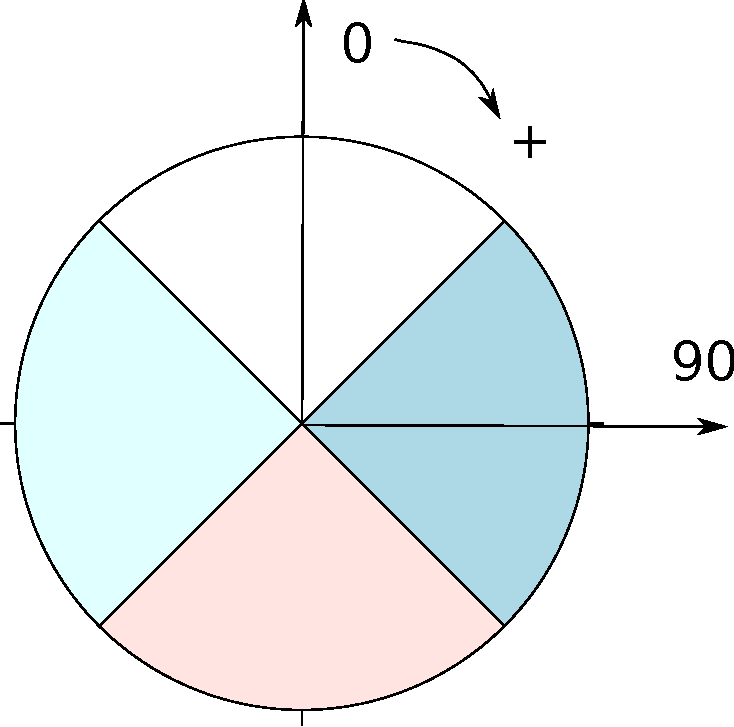
\includegraphics[width=1\textwidth]{./images/pic_1D/pie.pdf}
  \end{minipage}
\hspace{1.5cm}
  \begin{minipage}[c]{0.35\textwidth}
  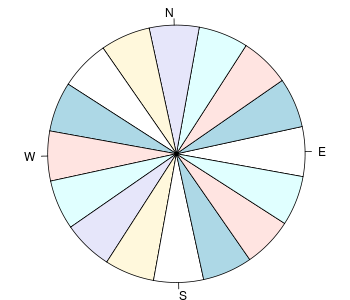
\includegraphics[width=1\textwidth]{./images/pic_1D/pie_16.png}
  \end{minipage}
\end{center}
\textsl{\caption{Example of Horizon classes: on the left are plotted the default 4 classes while on
 the right are plotted 16 classes}\label{hc}}
\end{figure}

\noindent The file meteo\_horizon has two columns: the first column refers to the azimuth (i.e. from 0 to 
360 degrees, 0 being North). The second column refers to the elevation of the obstacle in degrees 
(0 to 90, 0 meaning no obstacle). For example, if you are in a flat desert, for every azimuth degree you have always the elevation of the
obstacle=0 degrees.\\

\noindent If the file is not provided, by default an infinite horizon is considered
and the model creates that file with 4 horizon classes, as shown in \textsl{Figure \ref{azh}}.
\textsl{Figure \ref{hc}} shows the horizon classification with 16 classes.
Note that the North direction must always be
in the center of the slides in which the circle is divided.

%\noindent Let us call $\theta$ the azimuth and $\alpha$ the obstacle:
\begin{table}[!h]
\begin{center}
\begin{minipage}[c]{0.3\textwidth}
\begin{tabular}{c|c}
azimuth & obstacle\\
$\theta$ & $\alpha$\\
\hline
45 \textdegree	&	0.00\\
135 \textdegree	&	0.00\\
225 \textdegree	& 	0.00\\
315 \textdegree	&	0.00\\
\hline
\end{tabular}
\end{minipage}
%\hspace{0.5cm}
\begin{minipage}[c]{0.3\textwidth}
  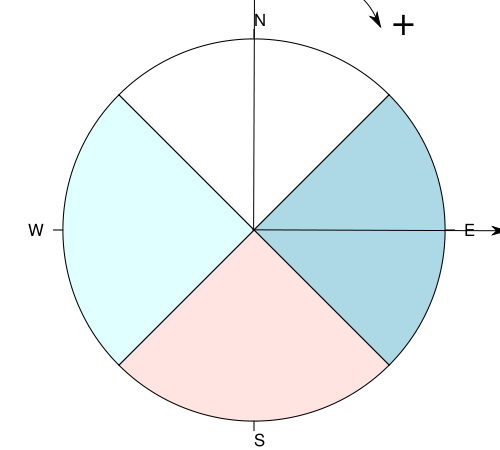
\includegraphics[width=1\textwidth]{./images/pic_1D/pie.png} 
\end{minipage}
\textsl{\caption{Example of the default horizon file and of the corresponding horizons classes}\label{azh}}
\end{center}
\end{table}




